\section{CONCEPTUAL DESIGN}
\subsection{Methodology} \label{sec:ConceptualDesignMethodology}
The conceptual design methodology for solar-powered UAVs used in this paper was developed at ETH Zurich by \cite{Noth_PhD,Leutenegger_JIRS} and is briefly summarized below. To analyze flight performance and a potential perpetual flight capability, the energy input/output-balance needs to be modeled. The total required electrical power
\begin{equation} \label{eqn:P_out}
P_{out,nom}=\frac{P_{level}}{\eta_{prop}}+P_{av}+P_{pld}
\end{equation}
consists of the required electrical propulsion power for level-flight $\frac{P_{level}}{\eta_{prop}}$ , where $\eta_{prop}$ includes propeller, gearbox, motor, and motor-controller efficiency, and the necessary avionics and payload power $P_{av}$ and $P_{pld}$. The aircraft is assumed to fly at the airspeed of minimum sink rate and thus minimum power consumption, i.e. its aerodynamic level-flight power is
\begin{equation} \label{eqn:P_level}
P_{level}=\left(\frac{C_D}{C_L^\frac{3}{2}}\right)_{min}\sqrt{\frac{2(m_{tot}g)^3}{\rho(h)A_{wing}}} .
\end{equation}
Here, $m_{tot}=m_{bat}+m_{struct}+m_{prop}+m_{sm}+m_{av}+m_{pld}$ is the total airplane mass, where structure, propulsion and solar module masses $m_{struct},m_{prop},m_{solar}$ are automatically sized according to \cite{Noth_PhD,Leutenegger_JIRS} and $m_{av},m_{pld}$ are given in table \ref{tab:ConceptDesignParameters}. The local earth gravity is designated by $g$, $A_{wing}$ is the wing area, and $rho$ is air density. The airplane lift and drag coefficients $C_L$ and $C_D$ are retrieved from 2-D airfoil simulations using XFoil \cite{Drela_XFoil}, with $C_D$ being combined with parasitic drag from the airplane fuselage and stabilizers and the induced drag  
\begin{equation} \label{eqn:C_D}
C_{D,ind}=\frac{c_L^2}{\pi\cdot e_0\cdot\lambda} .
\end{equation}
Here, $e_0\approx0.92$ is the Oswald efficiency and $\lambda$ is the wing aspect ratio. On the input side, the solar input power
\begin{equation} \label{eqn:P_solar}
P_{solar}=I\cdot A_{sm}\cdot\eta_{sm}\cdot\eta_{mppt}
\end{equation}
considers the solar module area $A_{sm}=ff_{sm}\cdot A_{wing}$ with relative fill-factor $ff_{sm}$, module efficiency $\eta_{sm}$, and Maximum Power Point Tracker (MPPT) efficiency $\eta_{mppt}$. The solar radiation $I=I(\varphi,h,t)$ is assumed to be a function of the geographical latitude $\varphi$, the altitude $h$, and the current date and local time $t$, and is modeled as in \cite{Duffie_SolarEngineering}.
The state equation can now be formulated in a simplified form as
\begin{equation}\label{eqn:StateEquations}
\begin{array}{r@{}l}
\frac{dE_{bat}}{dt}&=P_{solar}(\varphi,h,t)-u-P_{av}-P_{pld},\\
\frac{dh}{dt}&=\frac{\eta_{prop}\cdot u-P_{level}(h)}{m_{tot}g} .
\end{array}
\end{equation}
Here, $u$ is the actual electrical power sent to the propulsion system. Simple forward integration of the state equation (\ref{eqn:StateEquations}) gives the battery state of charge (SoC) over time and thus determines the perpetual flight capability.

For the design optimization, we assume that a solar-powered UAV configuration is designed for missions at and around a specific date of the year (DoY) and geographical latitude $\varphi$, and thus $\varphi$ and $DoY$ are fixed parameters. The three design parameters to be optimized are
\begin{itemize}
\item The wingspan $b$ and wing aspect ratio $\lambda$, which specify wing geometry and thus influence the level-power in (\ref{eqn:P_level}) and the solar input power in (\ref{eqn:P_solar}).
\item The battery mass $m_{bat}$ contained in $m_{tot}$ in (\ref{eqn:P_level}) 
\end{itemize}
\subsection{Extension of conceptual design optimization criteria}

The conceptual design tool developed in \cite{Noth_PhD,Leutenegger_JIRS} has been extended in two ways: First, it now provides the capability to perform energetic simulations of multi-day solar-powered flight, whereas before only one day-night cycle was considered. Fig. XXX shows the results for incoming solar power $P_{solar}$, required power $P_{elec,tot}$, and remaining battery charge $E_{bat}$ obtained for a two day/night cycle flight. Clearly, the initial charge condition $E_{bat}$ at $t=t_{sunrise}$ for the second day is different than on the first day, which significantly reduces the required charge time until $E_{bat}=E_{bat,max}=m_{bat}\cdot e_{bat}$ and leads to increased charge margins with respect to the pure one day/night-cycle simulation. %is this paragraph really needed?

\begin{figure}[tb]
    \centering
    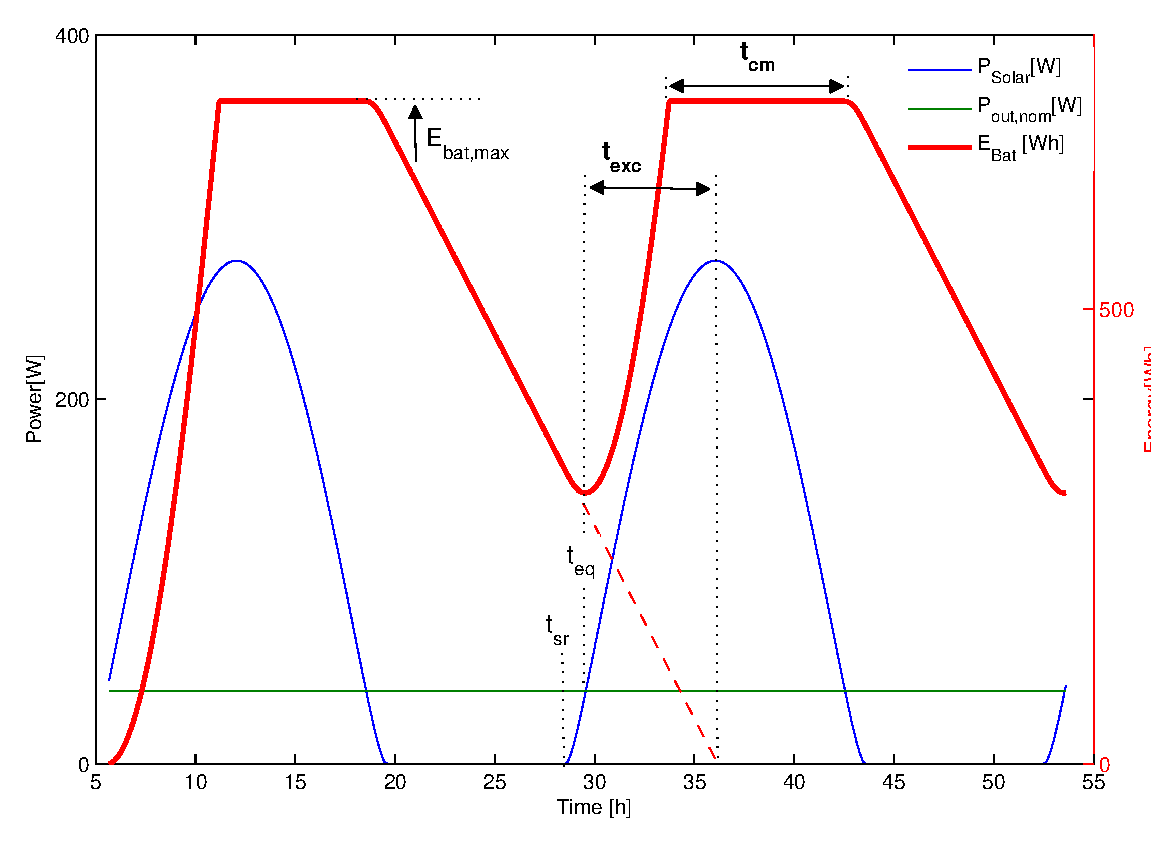
\includegraphics[width=\linewidth]{images/2_EnergySimulation}
    \caption{Energetic simulation of a specific UAV configuration (AtlantikSolar), showing input and output power, battery capacity, and performance metrics excess time $t_{exc}$ and charge margin $t_{cm}$ during a 2-day flight.}
    \label{fig:EnergySimulation}
\end{figure}

Second, and more importantly, the optimization criteria are extended with respect to \cite{Noth_PhD,Leutenegger_JIRS} to achieve more robust multi-day flight. In general, a necessary and sufficient condition for perpetual flight is that the excess time $t_{exc}>0$, i.e. that at $t=t_{eq}$ there exists remaining battery capacity to continue flight e.g. in case of cloud coverage in the morning. This is why\cite{Noth_PhD,Leutenegger_JIRS} focus on maximizing $t_{exc}$. However, a large $t_{exc}$ does not provide direct robustness against disturbances in $P_{solar}$ during the charging process(e.g. due to clouds). In contrast, when optimizing purely for $t_{exc}$, the methodology in sec. \ref{sec:ConceptualDesignMethodology} will select the largest battery size (due to the scaling of $P_{level}$ with $m_{bat}$ ) which can still be fully charged unter optimal conditions, but every reduction in $P_{solar}$ will directly decrease $t_{exc}$ due to only partially charged batteries. We thus introduce the charge margin $t_{cm}$ as the time margin between achieving the full charge $E_{bat}=E_{bat,max}$ and restart of the discharge in the evening. In case of decreased solar power income, $t_{cm}>0$ will provide an additional margin before a decrease in excess time occurs.

The overall approach for increasing robustness with respect to local disturbances in the power income and output is thus to determine the lowest acceptable $t_{exc}$ satisfying the UAV application requirements, and to then optimize the configuration for $t_{cm}$. The exact procedure applied here is:
\begin{itemize}
\item Choose the nominal operating latitude $\varphi$, the nominal Day-of-Operation $DoY_{nom}$, and the outermost days where perpetual UAV endurance is required $DoY_{min,max}$
\item Obtain $t_{night,min}$ and $t_{night,max}$ for the range of $DoY_{min,nom,max}$ from \cite{Duffie_SolarEngineering}. 
\item The required excess time $t_{exc,req}$ is now the sum of 
\begin{itemize}
	\item $t_{exc,DoY} = t_{night,max}-t_{night,min}$
	\item $t_{exc,clouds}$, to allow a margin for clouds in the morning or evening
	\item $t_{exc,P_{level}}$, to allow a margin for increased power consumption e.g. caused by downdrafts or uncertainties in estimating $P_{level}$
\end{itemize}
\item Perform the design analysis given the methodology in sec. \ref{sec:ConceptualDesignMethodology} for $DoY(t_{night}=t_{night,min})$. Pre-select the subset $\mathcal{S}$ of configurations satisfying $t_{exc}>t_{exc,req}$.
\item Within $\mathcal{S}$, choose the configuration $\mathcal{S}_i$ with the largest $t_{cm}$, taking into account UAV-specific further constraints on the design parameters $b$,$lambda$, or $m_{bat}$.
\end{itemize}

This conceptual design methodology is applied below. An alternative conceptual design approach utilizing a weighed version of $t_{exc}$ and $t_{cm}$ is proposed in \cite{Morton_ICRA2013}. 

% less predictable phenomenas such as clouds or winds. 
% local detoriation in the meteorological conditions. 
% AtlantikSolar charge curve is shown in figure above
% Explain(a simplified) POutput and PInput distrubance on this graphic. Name them (a) nominal (b) distrubed POutput (c) disturbed PInput. ???
% We need a mixture of both t_exc and t_cm, and how much we want to optimize exactly w.r.t the two depends on our confidence in the underlying performances. Power consumptino can be tested quite well, but meteo-conditions can not -> t\_cm very important, because t\_exc will then stay the same. If t\_cm is zero, no margin against bad meteo conditions. t\_exc should however still be on the order of some hours( we select t\_exc>~3hours), because this is how long clouds in morning/evening could/might cause P\_Solar~0. Also, minSoC>0.1, as this is limit for Go-Around-Operations.
% - optimizing only towards t\_exc will cause the method to select largest E\_bat which still results in full charge under the specific conditions
 
 \subsection{Application of Conceptual Design methodology} \label{sec:ConceptDesignApplication}
AtlantikSolar is designed for a nominal operating latitude of $\varphi=45°N$. It shall provide perpetual endurance within a +/-2 month window around $DoY_{nom}$=June 21\textsuperscript{st} (April 21\textsuperscript{st}-August 21\textsuperscript{st}). From \cite{Duffie_SolarEngineering}, we find $t_{night,min}=8.7h$ (June 21\textsuperscript{st}), $t_{night,max}=10.5h$(April 21\textsuperscript{st}), and thus $t_{exc,DoY}=1.80h$. We choose $t_{exc,clouds}=3.0h$ to account for three hours of full cloud coverage either on the evening or the morning and choose $t_{exc,P_{level}}=0.2\cdot t_{night,max}=2.1h$ to cover increased power consumption due to modelling errors, downdrafts or headwinds. Using $t_{exc,req}=t_{exc,DoY}+t_{exc,clouds}+t_{exc,P_{level}}$, we retrieve $t_{exc,req}=6.9h$ as the minimum required excess time for robust perpetual-flight at the given dates and locations. 

The design methodology tool of section \ref{sec:ConceptualDesignMethodology} is now applied assuming the fixed component performance parameters in Tab. \ref{tab:ConceptDesignParameters}. Fig. \ref{fig:ExcessTimeChargeMargin} shows the resulting plot for $t_{exc}$ versus the optimization variables wing span $b$, battery mass $m_{bat}$ and aspect ratio $\lambda=18.5$. The subset $\mathcal{S}$ of configurations satisfying $t_{exc}>t_{exc,req}$ is the region within the blue contour-line. The optimum clearly occurs at large wing spans, however, considering an external size constraint (each of the three wing pieces of AtlantikSolar shall be $<2m$ in wing span to allow proper handling and transport), we choose $b=5.6m$.  The aspect ratio $\lambda=18.5$ is found to provide an optimum in $t_{exc}$, and also allows to seamlessly integrate the solar cells (see section XXX) inside the wing chord. The last design choice is now $m_{bat}$, for which we seek to optimize $t_{cm}$ within the previously selected set $\mathcal{S}_1=(\mathcal{S}|b=5.6m, \lambda=18.5)$. As visible in Fig. \ref{fig:ExcessTimeChargeMargin}, $m_{bat}=3.0...7.5kg$ lie within $\mathcal{S}_1$. We choose $m_{bat}=3.5kg$ to optimize $t_{cm}$ and due to practical battery sizing constraints described in sec XXX. The selected configuration thus has an overall estimated mass of $m_{tot}=7.22kg$ and yields an estimated $t_{exc}=7.89h$ and $t_{cm}=8.38h$ for the nominal operating date and latitude.

\begin{figure}[tb]
    \centering
    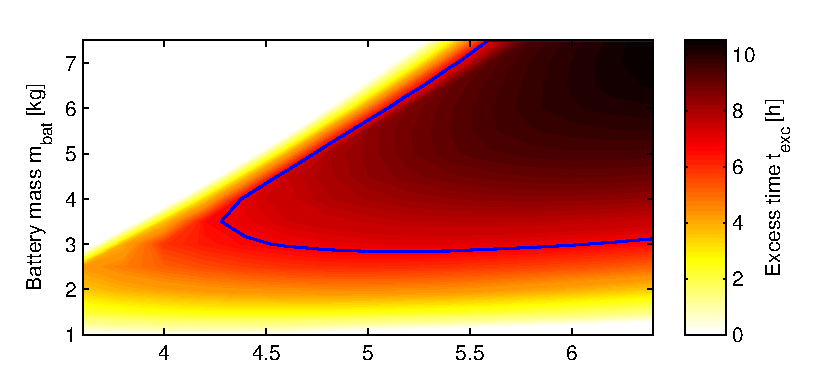
\includegraphics[width=\linewidth]{images/3_excesstime}
    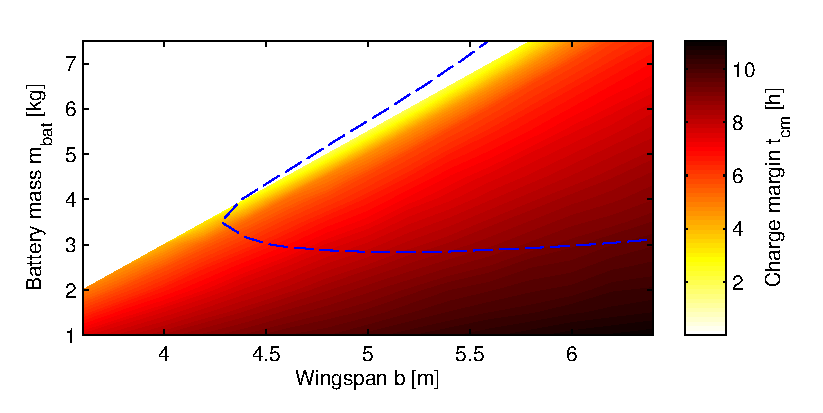
\includegraphics[width=\linewidth]{images/4_chargemargin}
    \caption{Excess time $t_{exc}$ (top) and charge margin $t_{cm}$ (bottom) vs. optimization parameters wingspan $b$ and $m_{bat}$, all at $\lambda=18.5$. The configuration subset $\mathcal{S}$ satisfying $t_{exc}>t_{exc,req}$ under our design requirements lies inside the blue contour line.}
    \label{fig:ExcessTimeChargeMargin}
\end{figure}

\begin{table}[h] 
\label{tab:ConceptDesignParameters}
\caption{Fixed parameters for the conceptual design}
\begin{center}
\begin{tabular}{l l l}
\hline Parameter & Value & Description\\ 
\hline $eta_{sm}$ & 0.20&Solar module efficiency\\
\hline $eta_{MPPT}$ & 0.97&MPPT efficiency\\
\hline $eta_{prop}$ & 0.58 &Propulsion system effiency\\
\hline $e_{bat}$ & 874800\unitfrac{J}{kg}&Battery specific energy\\
\hline $ff_{sm}$ & 0.94&Solar module fill factor\\
\hline $k_{sm}$ & 0.59$\unitfrac{kg}{m²}$ & Solar module areal density\\
\hline $m_{av}$ & 0.6kg&Avionics mass (including all cabling)\\
\hline $m_{pld}$ & 0.1kg&Payload mass\\
\hline $P_{av}$ & 4.5\unit{W}&Avionics power consumption\\
\hline $P_{pld}$ & 0.0\unit{W}&Payload power consumption\\
\end{tabular}
\end{center}
\end{table}

 \subsection{Robustness analysis}
To verify the multi-day flight robustness of the developed UAV configuration, we analyze its performance considering a set of local disturbances in UAV power input and output, namely
\begin{itemize}
\item The disturbed solar power income $P_{in,dist}$, as caused by various forms of clouds or fog. Lacking knowledge of the exact spatial and temporal cloud distribution, we'll assume the simple scaling $$ P_{in}(t) = P_{in,nom}(t) \cdot k_{CCF}. $$ Here, $k_{CCF}=[0,1]$  represents the current cloud cover factor \cite{Kimura_SolarRadAndClouds}, i.e. the clearness of the atmosphere.
\item The disturbed electrical power output $P_{out,dist}$. Wind downdrafts, head wind, or wind gusts may require increased propulsion or actuation power. Again, we'll assume the scaling  $$ P_{out}(t) = P_{out,nom}(t) \cdot k_{OPF}, $$ with OPF representing the Output Power Factor.
\end{itemize}
\begin{figure}
    \centering
    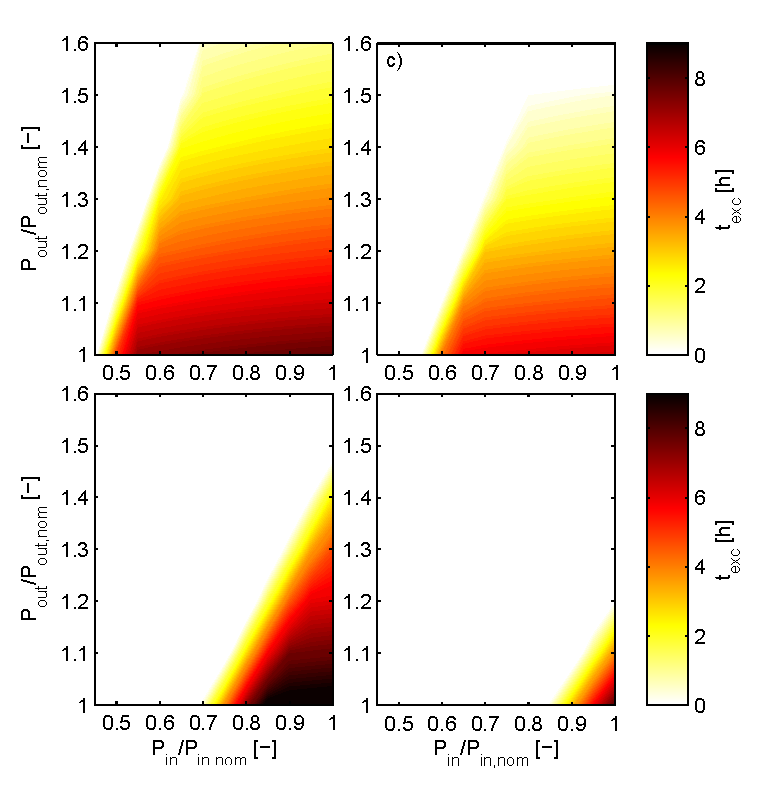
\includegraphics[width=\linewidth]{images/5_texcRobustness}
    \caption{Excess time $t_{exc}$ under disturbed power input and output for the developed $b=5.6m$, $\lambda=18.5$ configuration: a) $m_{bat}$=3.5kg on June 21\textsuperscript{st} b) $m_{bat}=6.0kg$ on June 21\textsuperscript{st} c) $m_{bat}$=3.5kg on April 21\textsuperscript{st} d) $m_{bat}=6.0kg$ on April 21\textsuperscript{st} }
    \label{fig:ExcessTimeRobustness}
\end{figure}
Fig. \ref{fig:ExcessTimeRobustness} shows the remaining excess time with respect to these disturbances. The UAV configuration developed in section \ref{sec:ConceptDesignApplication} (with $m_{bat}=3.5kg$) still provides perpetual endurance with less than 50\% of the solar power income or if more than 60\% surplus power are required e.g. to compensate for downdrafts on June 21\textsuperscript{st} (Fig.\ref{fig:ExcessTimeRobustness}a). In contrast, a configuation purely optimized towards excess time with $m_{bat}=6.0kg$ will yield a higher maximum $t_{exc}$ of 9.5h, however, the robustness with respect to clouds or higher required level power is greatly decreased (Fig.\ref{fig:ExcessTimeRobustness}b). On April  21\textsuperscript{st}, the UAV configuration of section \ref{sec:ConceptDesignApplication} still provides solid robustness, which verifies the +/-2month perpetual endurance requirement (Fig.\ref{fig:ExcessTimeRobustness}c). In contrast, the $m_{bat}=6.0kg$ configuratoin can not provide reliable perpetual endurance anymore (Fig.\ref{fig:ExcessTimeRobustness}d). This analysis verifies the advantages of the extended optimization criteria for achieving maximum robustness in perpetual endurance.